\documentclass[a4paper,14pt]{extreport}
  \usepackage[left=1.5cm,right=1.5cm,
      top=1.5cm,bottom=2cm,bindingoffset=0cm]{geometry}
  \usepackage{scrextend}
  \usepackage[T1,T2A]{fontenc}
  \usepackage[utf8]{inputenc}
  \usepackage[english,russian,ukrainian]{babel}
  \usepackage{tabularx}
  \linespread{1.5}
  \usepackage{amssymb}
  \usepackage{color}
  \usepackage{amsmath}
  \usepackage{mathrsfs}
  \usepackage{listings}
  \usepackage{graphicx}
  \graphicspath{ {./images/} }
  \usepackage{lipsum}
  \usepackage{xcolor}
  \usepackage{hyperref}
  \usepackage{tcolorbox}
  \usepackage{tikz}
  \usepackage[framemethod=TikZ]{mdframed}
  \usepackage{wrapfig,boxedminipage,lipsum}
  \mdfdefinestyle{MyFrame}{%
  linecolor=blue,outerlinewidth=2pt,roundcorner=20pt,innertopmargin=\baselineskip,innerbottommargin=\baselineskip,innerrightmargin=20pt,innerleftmargin=20pt,backgroundcolor=gray!50!white}
   \usepackage{csvsimple}
   \usepackage{supertabular}
  \usepackage{pdflscape}
  \usepackage{fancyvrb}
  %\usepackage{comment}
  \definecolor{ggreen}{rgb}{0.4,1,0}
  \definecolor{rred}{rgb}{1,0.1,0.1}
  \usepackage{array,tabularx}
  \usepackage{colortbl}

  \usepackage{varwidth}
  \tcbuselibrary{skins}
  \usepackage{fancybox}

  \definecolor{ggreen}{rgb}{0.4,1,0}
  \definecolor{rred}{rgb}{1,0.1,0.1}
  \definecolor{amber}{rgb}{1.0, 0.75, 0.0}
  \definecolor{babyblue}{rgb}{0.54, 0.81, 0.94}
  \definecolor{asparagus}{rgb}{0.53, 0.66, 0.42}
  \definecolor{chartreuse}{rgb}{0.5, 1.0, 0.0}
  \definecolor{darkorchid}{rgb}{0.6, 0.2, 0.8}
  \usepackage{fp}

  \usepackage{float}
  \usepackage{wrapfig}
  \usepackage{framed}
  %for nice Code{
  \lstdefinestyle{customc}{
    belowcaptionskip=1\baselineskip,
    breaklines=true,
    frame=L,
    xleftmargin=\parindent,
    language=C,
    showstringspaces=false,
    basicstyle=\small\ttfamily,
    keywordstyle=\bfseries\color{green!40!black},
    commentstyle=\itshape\color{purple!40!black},
    identifierstyle=\color{blue},
    stringstyle=\color{orange},
  }
  \lstset{escapechar=@,style=customc}
%}


\begin{document}

\newtcbox{\xmybox}[1][red]{on line, arc=7pt,colback=#1!10!white,colframe=#1!50!black, before upper={\rule[3pt] {0pt}{10pt}},boxrule=1pt,boxsep=0pt,left=6pt, right=6pt,top=2pt,bottom=2pt}


\pagecolor{white}
\begin{titlepage}
    \begin{center}
      \large
      Національний технічний університет України \\ "Київський політехнічний інститут імені Ігоря Сікорського"


      Факультет Електроніки

      Кафедра мікроелектроніки
      \vfill

      \textsc{ЗВІТ}\\

      {\Large про виконання практичної роботи №2\\
        з дисципліни: «Твердотільна електроніка-2»\\[1cm]

       

      }
    \bigskip
  \end{center}
  \vfill

  \newlength{\ML}
  \settowidth{\ML}{«\underline{\hspace{0.4cm}}» \underline{\hspace{2cm}}}
  \hfill
  \begin{minipage}{1\textwidth}
  Виконавець:\\
  Студент 3-го курсу \hspace{4cm} $\underset{\text{(підпис)}}{\underline{\hspace{0.2\textwidth}}}$  \hspace{1cm}А.\,С.~Мнацаканов\\
  \vspace{1cm}

  Перевірив: \hspace{6.1cm} $\underset{\text{(підпис)}}{\underline{\hspace{0.2\textwidth}}}$  \hspace{1cm}Л.\,М.~Королевич\\

  \end{minipage}

  \vfill

  \begin{center}
  2021
  \end{center}
\end{titlepage}


\centering{Схема зі спільною базою}
\begin{figure}[!h]
\caption{Схема включення зі спільною базою}
{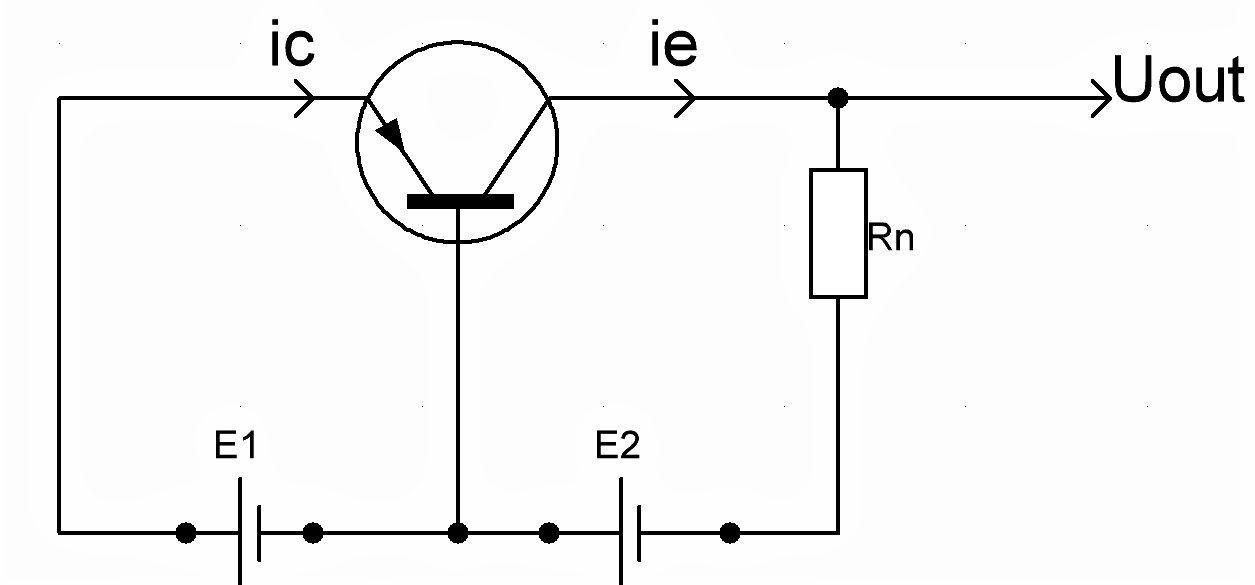
\includegraphics[width=0.7\textwidth]{combase}}
 \end{figure}

\begin{center}
$U_{out}=E_2-i_c\cdot{R_n}=i_c\cdot{R_c}$,\\[0.5cm]

$U_{in}=E_1=i_e\cdot{R_e}$,\\[0.5cm]

$K_U=\dfrac{U_{out}}{U_{in}}=\dfrac{i_c\cdot{R_c}}{i_e\cdot{R_e}}=\left|R_c>>R_e\right|\Rightarrow \boxed{K_U<<1}$\\[0.5cm]

$K_I=\dfrac{I_{out}}{I_{in}}=\dfrac{I_c}{I_e}=\left|I_c<I_e\right|\Rightarrow \boxed{K_I<1} (K_I\approx 0,95...0,99)$\\[0.5cm]
\end{center}
 
\newpage

\centering{Схема зі спільним колектором}
\begin{figure}[!h]
\caption{Схема включення зі спільним колектором}
{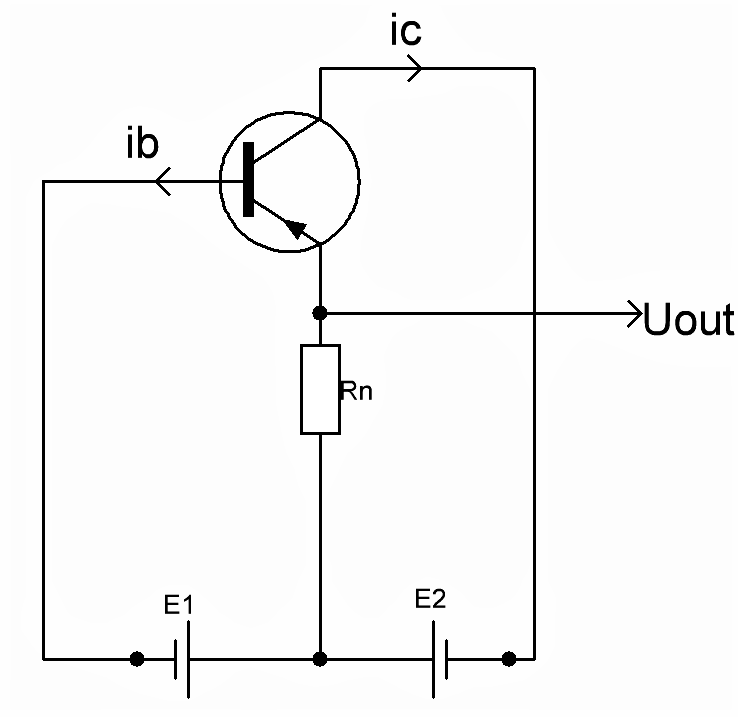
\includegraphics[width=0.5\textwidth]{comcol}}
 \end{figure}

\begin{center}
$U_{out}=-E_2+i_c\cdot{R_c}$\\[0.5cm]

$U_{in}=E_1=U_{out}+i_b\cdot{R_b}$\\[0.5cm]

$K_U=\dfrac{U_{out}}{U_{in}}=\dfrac{i_c\cdot{R_c}-E_2}{i_c\cdot{R_c}-E_2+i_b\cdot{R_b}}=\dfrac{U_{out}}{U_{out}+i_b\cdot{R_b}}\Rightarrow\boxed{K_U<1}$\\[0.5cm]

$K_I=\dfrac{I_{out}}{I_{in}}=\dfrac{I_e}{I_b}=\left|I_e>>I_b\right|\Rightarrow\boxed{K_I>>1}$
\end{center}
 
\newpage
\centering{Схема зі спільним емітером}
\begin{figure}[!h]
\caption{Схема включення зі спільним емітером}
{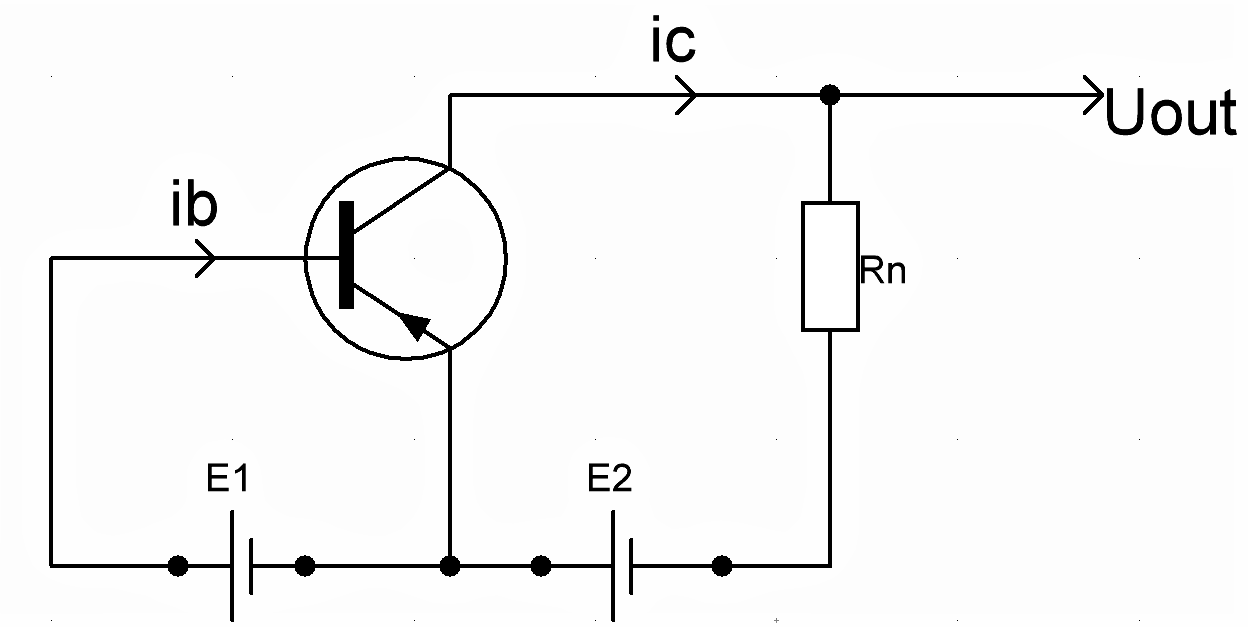
\includegraphics[width=0.7\textwidth]{comem}}
 \end{figure}

\begin{center}
$U_{out}=i_c\cdot{R_c}$\\[0.5cm]

$U_{in}=-i_b\cdot{R_b}$\\[0.5cm]

$K_U=\dfrac{U_{out}}{U_{in}}=-\dfrac{i_c\cdot{R_c}}{i_b\cdot{R_b}}=\left|R_c>>R_b\right|\Rightarrow\boxed{K_U>>1}$\\[0.5cm]

$K_I=\dfrac{I_{out}}{I_{in}}=\dfrac{I_c}{I_b}=\left|I_c>I_b\right|\Rightarrow\boxed{K_I>1}$
\end{center}

 
\newpage







 \centering{Схема зі спільним витоком}
\begin{figure}[!h]
\caption{Схема включення зі спільним витоком}}
{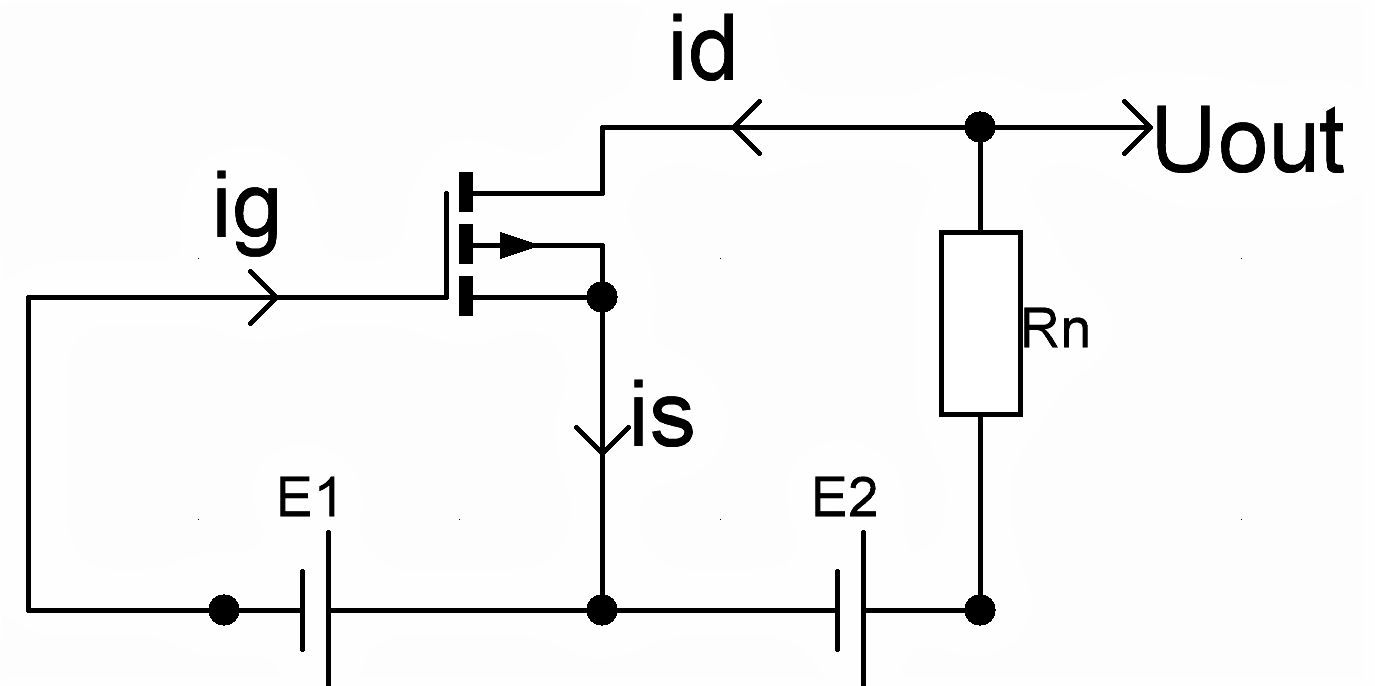
\includegraphics[width=0.7\textwidth]{comsource}
 \end{figure}

\begin{center}
Затвор ізольований $\Rightarrow R_g>>1$\\[0.5cm]

$E_2>E_1$\\[0.5cm]

$U_{out}=i_d\cdot{R_d}-E_2$\\[0.5cm]

$U_{in}=-i_g\cdot{R_g}$\\[0.5cm]

$K_U=\dfrac{U_{out}}{U_{in}}=\dfrac{i_d\cdot{R_d}-E_2}{-i_g\cdot{R_g}}=\left|R_g>>1, i_g\rightarrow 0\right|\Rightarrow\boxed{K_U>>1}$.
\end{center}
 
\newpage

\centering{Схема зі спільним стоком}
\begin{figure}[!h]
\caption{Схема включення зі спільним стоком}
{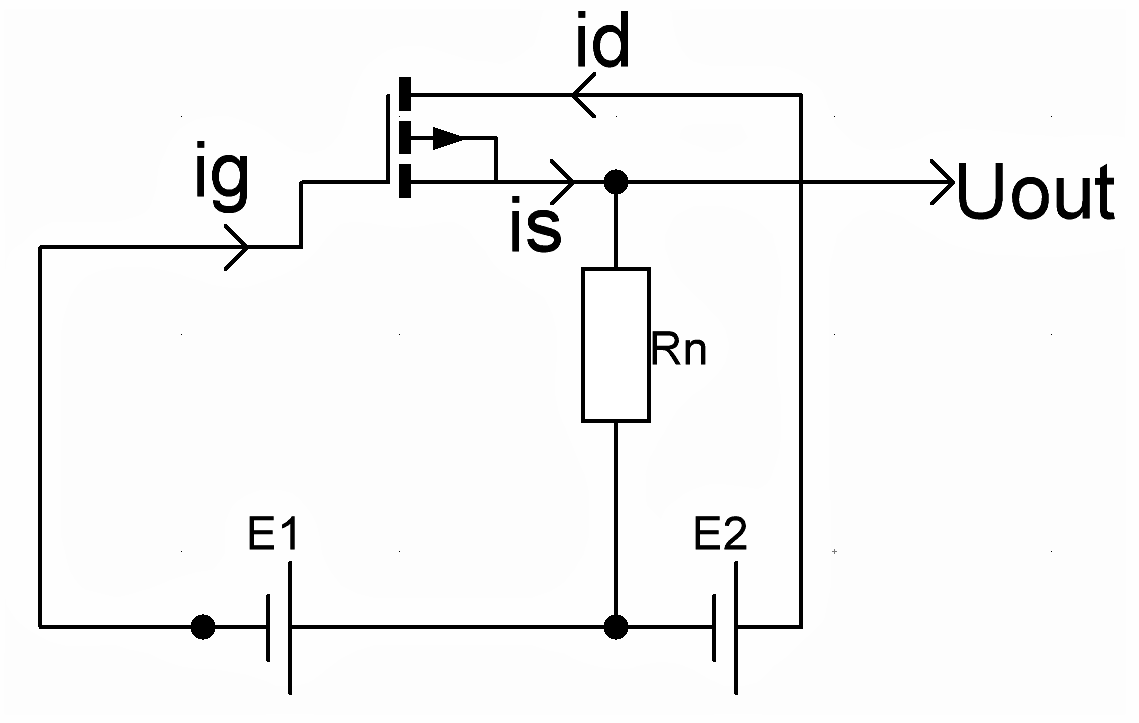
\includegraphics[width=0.7\textwidth]{comdrain}}
 \end{figure}

\begin{center}
$U_{out}=E_2-i_s\cdot{R_s}$\\[0.5cm]

$U_{in}=-R_n\cdot{i_s}-i_g\cdot{R_g}$\\[0.5cm]

$K_U=\dfrac{U_{out}}{U_{in}}=\dfrac{E_2-i_s\cdot{R_s}}{-R_n\cdot{i_s}-i_g\cdot{R_g}}\approx 1$
\end{center}
 
\newpage

\centering{Схема зі спільним затвором}
\begin{figure}[!h]
\caption{Схема включення зі спільним затвором}
{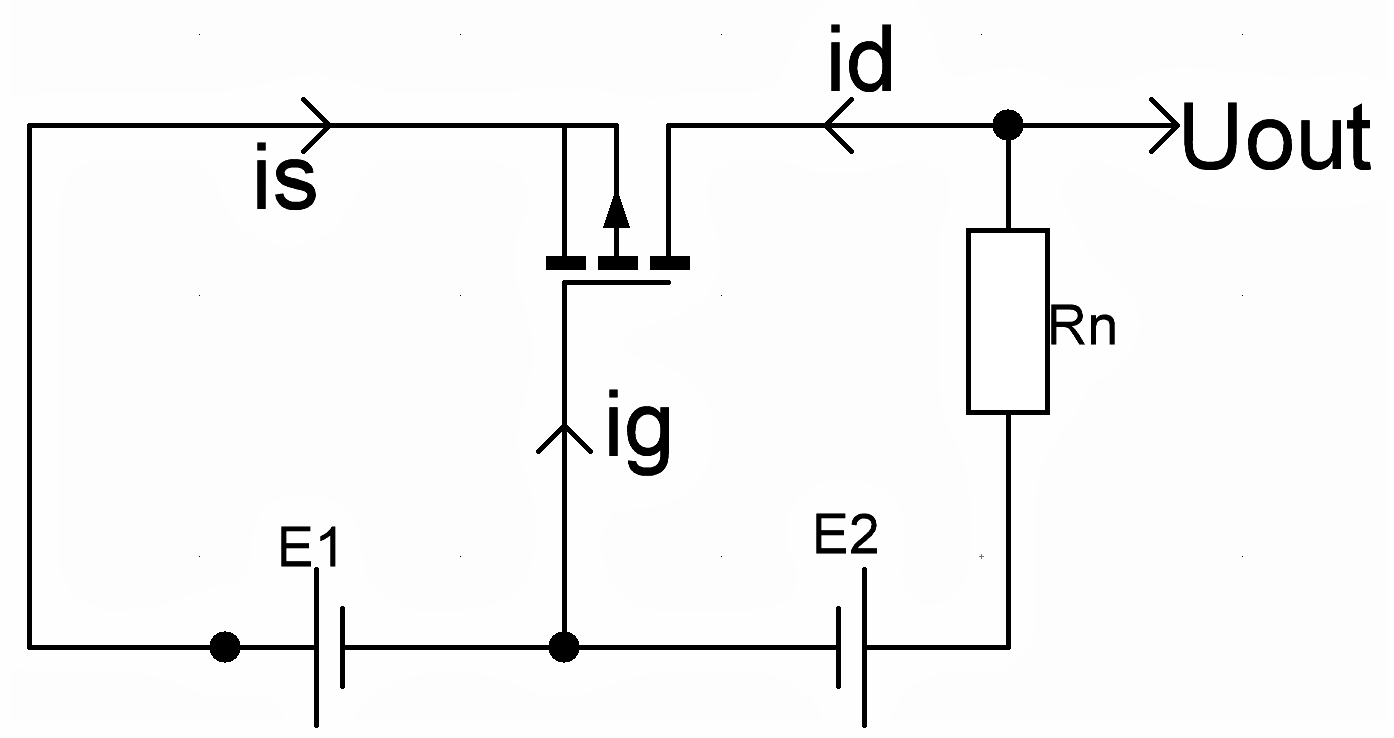
\includegraphics[width=0.7\textwidth]{comgate}}
 \end{figure}


\begin{center}
$U_{out}=i_d\cdot{R_n}+i_d\cdot{R_d}$\\[0.5cm]

$U_{in}=i_s\cdot{R_s}$\\[0.5cm]

$K_U=\dfrac{U_{out}}{U_{in}}=\dfrac{i_d\cdot{R_n}+i_d\cdot{R_d}}{i_s\cdot{R_s}}>1$
\end{center}










\end{document}
